%\section{Construction of Discrete-Time  Queueing Processes}
\section{Queueing Processes in Discrete-Time}
\label{sec:constr-discr-time}


\opt{solutionfiles}{
\Opensolutionfile{hint}
\Opensolutionfile{ans}
}

We start with a description of a case to provide motivation to study queueing systems.
Then we develop a set of recursions of fundamental importance to construct and simulate queueing systems.
With these recursions, we analyze the efficacy of several suggestions to improve the case system.
To illustrate the power of this approach, we close the section with a large number of exercises in which you develop recursions for many different queueing situations.

\subsection*{Case}
\label{sec:case}

At a mental health department, five psychiatrists do intakes of future patients to determine the best treatment process for the patients.
There are complaints about the time patients have to wait for their first intake; the desired waiting time is around two weeks, but the realized waiting time is sometimes more than three months.
The organization considers this to be unacceptably long, but\ldots what to do about it?

To reduce the waiting times, the five psychiatrists have various
suggestions. 
\begin{enumerate}
\item Not all psychiatrists have the same amount of time available per week to do intakes.
  This is not a problem during weeks when all psychiatrists are present; however, psychiatrists tend to take holidays, visit conferences, and so on.
  So, if the psychiatrist with the most intakes per week would go on leave, this might affect the behavior of the queue length considerably.
  This raises the question about the difference in the allocation of capacity allotted to the psychiatrists.
  What are the consequences on the distribution and average of the waiting times if they would all have the same weekly capacity?
\item The psychiatrists tend to plan their holidays consecutively, to reduce the variation in the service capacity.
  What if they would synchronize their holidays, to the extent possible, rather than spread their holidays?
\item Finally, suppose the psychiatrists would do 2 more intakes per week in busy times and 2 fewer in quiet weeks.
  Assuming that the system is stable, i.e., the average service capacity is larger than the average demand, then on average the psychiatrists would not do more intakes, i.e., their workload would not increase, but the queue length may be controlled better.
\end{enumerate}

As this case is too hard to analyze by mathematical means,  we need to develop a model to simulate the queueing system in discrete time. 
With this simulator we can evaluate the effect of these suggestions on reducing the queueing dynamics.
%we need to develop a simple simulator with which we can make a number of plots.
Interestingly, the structure of the simulation is very simple, so simple that it is also an exceedingly convincing tool to communicate the results of an analysis of a queueing system to managers (and the like).

\subsection*{Recursions}

Let us start with discussing the essentials of the simulation of a queueing system.
The easiest way to construct queueing processes is to `chop up' time in periods and develop recursions for the behavior of the queue from period to period.
Using fixed-sized periods has the advantage that we do not have to specify specific inter-arrival times or service times of individual customers; only the number of arrivals in a period and the number of potential services are relevant.
Note that the length of such a period depends on the context for which the model is developed.
For instance, to study queueing processes at a supermarket, a period can consist of $5$ minutes, while for a production environment, e.g., a job shop, it can be a day, or even a week.


Let us define:
\begin{itemize}
    \item[$a_k =$] number of jobs that arrive \textit{in} period $k$,
    \item[$c_k= $] the capacity, i.e., the maximal number of jobs that can be served, during period~$k$,
    \item[$d_k =$] number of jobs that depart \textit{in} period $k$,
    \item[$L_k =$] number of jobs in the system at the \textit{end} of period $k$.
\end{itemize}
% \begin{equation}
%   \label{eq:30}
%   \begin{split}
%     a_k &= \text{number of jobs that arrive \textit{in} period $k$},\\
%     c_k &= \text{the capacity, i.e., the maximal number of jobs that can be served, during period $k$},\\
%     d_k &= \text{number of jobs that depart  \textit{in} period $k$},\\
%     L_k &= \text{number of jobs in the system  at the \textit{end} of period $k$}.\\
%   \end{split}
% \end{equation}
In the sequel we also call $a_k$ the \emph{size of the batch} arriving in period $k$.
Note that the definition of $a_k$ is a bit subtle: we may assume that the arriving jobs arrive either at the start or at the end of the period.
In the first case, the jobs can be served in period $k$, in the latter case, they \emph{cannot} be served in period~$k$.


Since $L_{k-1}$ is the queue length at the \emph{end} of period $k-1$, it must also be the number of customers at the \emph{start} of period $k$.
Assuming that jobs arriving in period $k$ cannot be served in period~$k$, the number of customers that depart in period $k$ is
\begin{subequations}\label{eq:31}
\begin{equation}\label{eq:d_k}
d_k = \min\{L_{k-1}, c_k\},
\end{equation}
since only the jobs that are present at the start of the period, i.e., $L_{k-1}$, can be served if the capacity exceeds the queue length.
Now that we know the number of departures, the number at the end of period $k$ is given by
\begin{equation}
    L_k = L_{k-1} -d_k + a_k.
\end{equation}
\end{subequations}
Like this, if we are given $L_0$,  we can obtain $L_1$, and from this  $L_2$, and so on.

Note that in this type of queueing system there is not a job in service, we only count the jobs in the system at the end of a period. Thus, the number of jobs in the system and in queue coincide in this model.

\begin{extra}
Suppose that $c_k= 7$ for all $k$, and $a_1=5$, $a_2=4$
and $a_3=9$; also $L_0=8$. What are $d_k$ and $L_k$ for $k\geq 1$? 
\begin{solution}
$d_1=7$, $L_1=8-7+5=6$, $d_2 = 6$,
$L_2=6-6+4=4$, $d_3 = 4$, $L_3=4-4+9=9$, and so on. 
\end{solution}
\end{extra}

\begin{extra}
 What is the interpretation of setting
    $d_k = \min\{L_{k-1}+a_k,  c_k\}$ rather than definition~\cref{eq:d_k}?
\begin{solution}
 The assumption is that the jobs arrive at the start of period
    $k$, before service in period $k$ starts, rather than at the end
    of the period. Therefore the arrivals at period $k$ can also be
    served during period $k$.
\end{solution}
\end{extra}


\begin{exercise}\clabel{ex:24}
  Show that the scheme
\begin{equation}\label{eq:5}
  \begin{split}
  L_k &= [L_{k-1}+a_k - c_k]^+,\\
  d_k &= L_{k-1} +a_k- L_{k}.
  \end{split}
\end{equation}
is equivalent to a modification of~\cref{eq:31} in which we assume that jobs can be served in the period they arrive.
\begin{solution}
Starting from ,
  \begin{align*}
    d_k &= \min\{L_{k-1}+a_k, c_k\}, \\
    L_k &= L_{k-1} + a_k - d_k,
  \end{align*}
  we get
  \begin{align*}
    L_k &= L_{k-1} + a_k - d_k \\ 
        &= L_{k-1} + a_k - \min\{L_{k-1}+a_k, c_k\} \\
        &= \max\{L_{k-1} + a_k - c_k, 0 \}.
  \end{align*}
\end{solution}
\end{exercise}



Of course we are not going to carry out these computations by hand.
Typically we use company data to model the arrival process $\{a_k\}_{k=1,2,\ldots}$ and the capacity $\{c_k\}_{k=1,2,\ldots}$ and feed this data into a computer to carry out the recursions~\cref{eq:31}.
If we do not have sufficient data, we make a probability model for these data and use the computer to generate random numbers with, hopefully, similar characteristics as the real data.
At any rate, from this point on, we assume that it is easy, by means of computers, to obtain numbers $a_1,\ldots, a_n$ for $n\gg 1000$, and so on.


\subsection*{Case analysis}
\label{sec:case-analysis}

Here we continue with the case of the five psychiatrists and analyze the proposed rules to improve the performance of the system.
We mainly want to reduce the long waiting times.

As a first step in the analysis, we model the arrival process of patients as a Poisson process, cf.~\cref{sec:poisson-distribution}.
The duration of a period is taken to be a week.
The average number of arrivals per period, based on data of the company, was slightly less than~12 per week; in the simulation we set it to $\lambda= 11.8$ per week.
We model the capacity in the form of a matrix such that row $i$ corresponds to the weekly capacity of psychiatrist $i$:
\begin{equation*}
C = 
  \begin{pmatrix}
    1 & 1 & 1 & \ldots\\
    1 & 1 & 1 & \ldots\\
    1 & 1 & 1 & \ldots\\
    3 & 3 & 3 & \ldots\\
    9 & 9 & 9 & \ldots\\
  \end{pmatrix}.
\end{equation*}
Thus, psychiatrists 1, 2, and 3 do just one intake per week, the
fourth does 3, and the fifth does 9 intakes per week. The sum over
column $k$ is the total service capacity for week $k$ of all
psychiatrists together.

With the matrix $C$ it is simple to make other capacity schemes. A
more balanced scheme would be like this:
\begin{equation*}
C = 
  \begin{pmatrix}
    2 & 2 & 2 & \ldots\\
    2 & 2 & 2 & \ldots\\
    3 & 3 & 3 & \ldots\\
    4 & 4 & 4 & \ldots\\
    4 & 4 & 4 & \ldots\\
  \end{pmatrix}.
\end{equation*}

Next, we include the effects of holidays on the capacity. This is
easily done by setting the capacity of a certain psychiatrist to~$0$ in
a certain week. Let us assume that just one psychiatrist is on leave in
a week, each psychiatrist has one week per five weeks off, and the
psychiatrists' holiday schemes rotate. To model this, we set
$C_{1,1}=C_{2,2}=\cdots=C_{1,6}=C_{2,7} =\cdots = 0$, i.e.,
\begin{equation*}
C = 
  \begin{pmatrix}
    0 & 2 & 2 & 2 & 2 & 0 & \ldots \\
    2 & 0 & 2 & 2 & 2 & 2 & \ldots\\
    3 & 3 & 0 & 3 & 3 & 3 & \ldots\\
    4 & 4 & 4 & 0 & 4 & 4 & \ldots\\
    4 & 4 & 4 & 4 & 0 & 4 & \ldots\\
  \end{pmatrix}.
\end{equation*}
Hence, the total average capacity must be $4/5 \cdot (2+2+3+4+4) = 12$
patients per week.  The other holiday scheme---all psychiatrists take
holiday in the same week--corresponds to setting entire columns to
zero, i.e., $C_{i,5}=C_{i,10}=\cdots=0$ for week $5$, $10$, and so
on. Note that all these variations in holiday schemes result in the
same average capacity.

Now that we have modeled the arrivals and the capacities, we can use the recursions~\cref{eq:31} to simulate the queue length process for the four different scenarios proposed by the psychiatrists, unbalanced versus balanced capacity, and spread out holidays versus simultaneous holidays.

The results are shown in~\cref{fig:balanced}.
It is apparent that Suggestions 1 and 2 above do not significantly affect the behavior of the queue length process.



\begin{figure}[ht]
  \centering
% progs/intake_control.py
% This file was created by tikzplotlib v0.9.1.
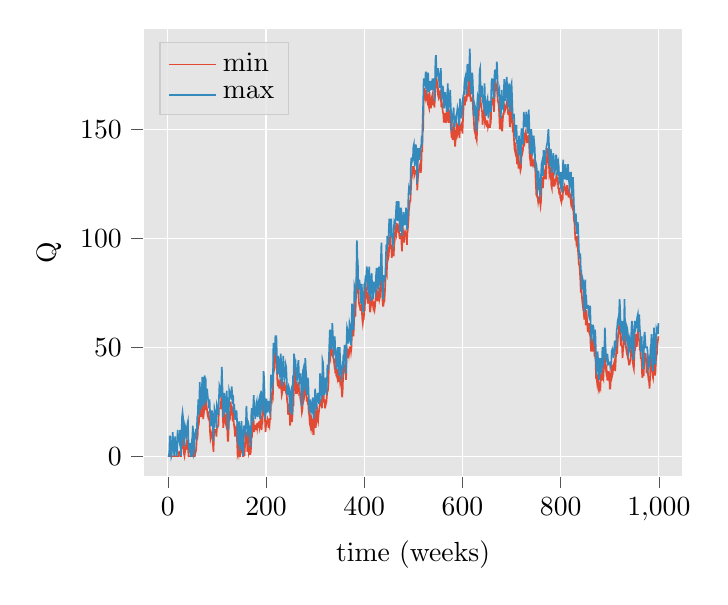
\begin{tikzpicture}

\definecolor{color0}{rgb}{0.886274509803922,0.290196078431373,0.2}
\definecolor{color1}{rgb}{0.203921568627451,0.541176470588235,0.741176470588235}

\begin{axis}[
axis background/.style={fill=white!89.8039215686275!black},
axis line style={white},
legend cell align={left},
legend style={fill opacity=0.8, draw opacity=1, text opacity=1, at={(0.03,0.97)}, anchor=north west, draw=white!80!black, fill=white!89.8039215686275!black},
tick align=outside,
tick pos=left,
x grid style={white},
xlabel={time (weeks)},
xmajorgrids,
xmin=-49.95, xmax=1048.95,
xtick style={color=white!33.3333333333333!black},
y grid style={white},
ylabel={Q},
ymajorgrids,
ymin=-9.35, ymax=196.35,
ytick style={color=white!33.3333333333333!black}
]
\addplot [semithick, color0]
table {%
0 0
1 0
2 0
3 0
4 0
5 1
6 0
7 0
8 0
9 0
10 0
11 0
12 0
13 0
14 0
15 0
16 0
17 0
18 0
19 0
20 0
21 0
22 0
23 2
24 2
25 1
26 0
27 0
28 7
29 6
30 15
31 15
32 8
33 1
34 0
35 2
36 3
37 5
38 6
39 7
40 3
41 6
42 0
43 0
44 0
45 0
46 0
47 0
48 0
49 0
50 0
51 7
52 0
53 0
54 0
55 0
56 2
57 2
58 4
59 8
60 8
61 10
62 18
63 14
64 18
65 24
66 19
67 21
68 18
69 20
70 26
71 27
72 17
73 19
74 21
75 27
76 25
77 28
78 21
79 23
80 21
81 19
82 18
83 19
84 18
85 16
86 11
87 8
88 9
89 10
90 11
91 10
92 5
93 2
94 10
95 12
96 12
97 12
98 11
99 9
100 13
101 13
102 14
103 14
104 22
105 22
106 22
107 22
108 22
109 29
110 31
111 24
112 18
113 13
114 16
115 19
116 18
117 16
118 15
119 19
120 20
121 13
122 7
123 7
124 13
125 20
126 20
127 19
128 25
129 22
130 22
131 20
132 16
133 23
134 16
135 14
136 12
137 9
138 12
139 13
140 11
141 7
142 1
143 2
144 1
145 6
146 0
147 0
148 2
149 4
150 8
151 5
152 2
153 0
154 0
155 2
156 0
157 4
158 11
159 9
160 11
161 8
162 2
163 11
164 9
165 2
166 3
167 1
168 1
169 2
170 7
171 12
172 11
173 14
174 17
175 16
176 11
177 14
178 14
179 14
180 12
181 15
182 13
183 15
184 15
185 13
186 16
187 13
188 14
189 18
190 18
191 12
192 18
193 17
194 22
195 27
196 26
197 22
198 16
199 11
200 14
201 16
202 16
203 17
204 16
205 13
206 15
207 14
208 17
209 17
210 25
211 27
212 26
213 29
214 28
215 40
216 39
217 40
218 45
219 49
220 43
221 45
222 40
223 35
224 32
225 34
226 33
227 31
228 34
229 35
230 35
231 31
232 28
233 29
234 31
235 34
236 30
237 32
238 33
239 31
240 30
241 31
242 29
243 25
244 24
245 19
246 22
247 24
248 19
249 14
250 17
251 20
252 16
253 16
254 19
255 25
256 23
257 40
258 42
259 38
260 32
261 29
262 29
263 32
264 31
265 30
266 34
267 31
268 31
269 29
270 26
271 25
272 23
273 20
274 21
275 27
276 30
277 26
278 27
279 32
280 33
281 30
282 30
283 25
284 27
285 24
286 24
287 20
288 19
289 15
290 14
291 13
292 18
293 17
294 14
295 15
296 10
297 10
298 18
299 18
300 19
301 13
302 15
303 20
304 21
305 17
306 16
307 19
308 21
309 23
310 26
311 23
312 25
313 24
314 22
315 32
316 33
317 31
318 25
319 25
320 22
321 26
322 24
323 25
324 28
325 30
326 30
327 33
328 42
329 46
330 46
331 45
332 51
333 46
334 49
335 49
336 46
337 45
338 44
339 42
340 43
341 38
342 40
343 37
344 37
345 36
346 40
347 36
348 34
349 37
350 38
351 34
352 35
353 34
354 30
355 27
356 30
357 37
358 40
359 41
360 39
361 39
362 38
363 35
364 46
365 47
366 48
367 45
368 49
369 47
370 49
371 50
372 50
373 48
374 50
375 58
376 56
377 57
378 55
379 60
380 66
381 67
382 64
383 72
384 77
385 87
386 81
387 82
388 74
389 71
390 69
391 69
392 67
393 67
394 69
395 67
396 63
397 61
398 63
399 63
400 67
401 67
402 74
403 80
404 74
405 75
406 75
407 70
408 73
409 72
410 75
411 69
412 66
413 68
414 71
415 72
416 69
417 71
418 69
419 71
420 68
421 67
422 69
423 72
424 77
425 74
426 76
427 71
428 74
429 74
430 75
431 72
432 73
433 79
434 85
435 86
436 77
437 72
438 69
439 69
440 71
441 71
442 75
443 80
444 85
445 85
446 84
447 94
448 96
449 91
450 92
451 99
452 100
453 101
454 95
455 97
456 91
457 93
458 94
459 92
460 92
461 97
462 99
463 104
464 103
465 102
466 107
467 104
468 105
469 104
470 105
471 102
472 100
473 100
474 102
475 102
476 97
477 94
478 106
479 103
480 100
481 98
482 102
483 103
484 102
485 102
486 100
487 97
488 106
489 105
490 108
491 113
492 115
493 117
494 117
495 122
496 127
497 128
498 133
499 130
500 130
501 133
502 129
503 130
504 131
505 131
506 131
507 128
508 122
509 127
510 129
511 131
512 132
513 133
514 134
515 130
516 132
517 140
518 140
519 149
520 150
521 163
522 166
523 169
524 165
525 164
526 166
527 168
528 165
529 163
530 164
531 161
532 160
533 167
534 162
535 160
536 160
537 164
538 165
539 166
540 161
541 163
542 162
543 160
544 165
545 170
546 174
547 171
548 172
549 170
550 166
551 165
552 167
553 166
554 165
555 164
556 168
557 160
558 162
559 160
560 158
561 157
562 153
563 157
564 157
565 155
566 153
567 156
568 155
569 157
570 159
571 155
572 153
573 158
574 157
575 156
576 152
577 149
578 146
579 151
580 145
581 147
582 153
583 151
584 145
585 142
586 145
587 146
588 153
589 152
590 148
591 149
592 151
593 149
594 146
595 152
596 152
597 151
598 152
599 151
600 148
601 154
602 159
603 163
604 165
605 161
606 164
607 163
608 163
609 165
610 168
611 167
612 165
613 172
614 174
615 175
616 165
617 163
618 163
619 163
620 164
621 162
622 157
623 155
624 150
625 149
626 150
627 146
628 146
629 145
630 150
631 155
632 157
633 156
634 161
635 165
636 168
637 160
638 162
639 159
640 158
641 152
642 157
643 158
644 154
645 159
646 153
647 154
648 153
649 153
650 151
651 154
652 151
653 152
654 152
655 151
656 151
657 156
658 155
659 165
660 161
661 163
662 163
663 164
664 158
665 162
666 167
667 170
668 171
669 169
670 169
671 166
672 163
673 162
674 161
675 156
676 150
677 153
678 152
679 156
680 156
681 149
682 154
683 157
684 157
685 161
686 160
687 159
688 160
689 161
690 162
691 160
692 160
693 157
694 157
695 159
696 153
697 151
698 161
699 164
700 159
701 155
702 151
703 152
704 149
705 145
706 141
707 140
708 144
709 140
710 140
711 134
712 137
713 138
714 132
715 135
716 134
717 133
718 131
719 132
720 138
721 140
722 139
723 140
724 144
725 146
726 142
727 148
728 148
729 149
730 146
731 144
732 144
733 145
734 147
735 147
736 142
737 137
738 136
739 133
740 138
741 137
742 133
743 136
744 134
745 135
746 134
747 135
748 133
749 127
750 122
751 123
752 119
753 119
754 117
755 119
756 116
757 118
758 117
759 115
760 117
761 124
762 128
763 126
764 123
765 128
766 130
767 127
768 131
769 132
770 127
771 132
772 136
773 141
774 141
775 138
776 134
777 129
778 130
779 131
780 129
781 124
782 123
783 130
784 131
785 127
786 124
787 124
788 127
789 127
790 126
791 128
792 129
793 126
794 128
795 123
796 123
797 120
798 123
799 119
800 118
801 120
802 117
803 118
804 118
805 124
806 122
807 123
808 124
809 123
810 122
811 120
812 120
813 124
814 124
815 122
816 119
817 119
818 121
819 120
820 118
821 120
822 116
823 117
824 115
825 116
826 112
827 108
828 108
829 103
830 99
831 101
832 98
833 99
834 101
835 95
836 92
837 88
838 88
839 85
840 81
841 75
842 78
843 74
844 71
845 69
846 70
847 66
848 63
849 63
850 69
851 60
852 67
853 65
854 62
855 57
856 59
857 58
858 61
859 59
860 57
861 51
862 48
863 51
864 52
865 48
866 50
867 52
868 50
869 46
870 46
871 44
872 36
873 36
874 34
875 36
876 35
877 31
878 32
879 31
880 33
881 32
882 38
883 35
884 35
885 38
886 37
887 36
888 41
889 43
890 47
891 42
892 40
893 42
894 38
895 35
896 35
897 35
898 39
899 37
900 31
901 31
902 35
903 40
904 42
905 37
906 38
907 41
908 42
909 43
910 41
911 39
912 43
913 48
914 52
915 47
916 52
917 56
918 57
919 60
920 60
921 58
922 53
923 54
924 51
925 50
926 45
927 49
928 50
929 55
930 60
931 51
932 53
933 50
934 48
935 47
936 48
937 45
938 44
939 42
940 42
941 43
942 44
943 47
944 52
945 50
946 49
947 43
948 41
949 40
950 46
951 52
952 51
953 56
954 53
955 50
956 54
957 58
958 54
959 54
960 53
961 49
962 49
963 45
964 45
965 43
966 36
967 38
968 37
969 37
970 43
971 47
972 47
973 47
974 44
975 38
976 40
977 41
978 37
979 35
980 34
981 31
982 36
983 47
984 45
985 44
986 40
987 37
988 36
989 43
990 47
991 43
992 37
993 39
994 44
995 46
996 47
997 51
998 53
999 55
};
\addlegendentry{min}
\addplot [semithick, color1]
table {%
0 0
1 0
2 0
3 2
4 9
5 9
6 3
7 0
8 1
9 4
10 11
11 6
12 4
13 0
14 5
15 9
16 5
17 3
18 0
19 2
20 12
21 9
22 8
23 7
24 6
25 12
26 7
27 0
28 11
29 18
30 20
31 18
32 8
33 5
34 5
35 14
36 13
37 12
38 10
39 12
40 15
41 16
42 7
43 4
44 3
45 6
46 4
47 0
48 0
49 7
50 9
51 14
52 4
53 1
54 2
55 10
56 11
57 10
58 9
59 12
60 18
61 19
62 26
63 19
64 22
65 34
66 28
67 29
68 23
69 24
70 36
71 36
72 25
73 24
74 25
75 37
76 34
77 36
78 26
79 27
80 31
81 28
82 26
83 24
84 22
85 26
86 20
87 16
88 14
89 14
90 21
91 19
92 13
93 7
94 14
95 22
96 21
97 20
98 16
99 13
100 23
101 22
102 22
103 19
104 26
105 32
106 31
107 30
108 27
109 33
110 41
111 33
112 26
113 18
114 20
115 29
116 27
117 24
118 20
119 23
120 30
121 22
122 15
123 12
124 17
125 30
126 29
127 27
128 30
129 26
130 32
131 29
132 24
133 28
134 20
135 24
136 21
137 17
138 17
139 17
140 21
141 16
142 9
143 7
144 5
145 16
146 9
147 3
148 3
149 13
150 16
151 11
152 5
153 0
154 6
155 14
156 10
157 11
158 14
159 15
160 23
161 18
162 9
163 14
164 15
165 14
166 13
167 8
168 4
169 8
170 19
171 22
172 18
173 17
174 23
175 28
176 21
177 21
178 17
179 20
180 24
181 25
182 20
183 18
184 21
185 25
186 26
187 20
188 17
189 24
190 30
191 22
192 25
193 20
194 28
195 39
196 36
197 29
198 19
199 17
200 26
201 26
202 23
203 20
204 22
205 25
206 25
207 21
208 20
209 23
210 37
211 37
212 33
213 32
214 34
215 52
216 49
217 47
218 48
219 55
220 55
221 55
222 47
223 38
224 38
225 46
226 43
227 38
228 37
229 41
230 47
231 41
232 35
233 32
234 37
235 46
236 40
237 39
238 36
239 37
240 42
241 41
242 36
243 28
244 30
245 31
246 32
247 31
248 22
249 20
250 29
251 30
252 23
253 19
254 25
255 37
256 33
257 47
258 45
259 44
260 44
261 39
262 36
263 35
264 37
265 42
266 44
267 38
268 34
269 35
270 38
271 35
272 30
273 23
274 27
275 39
276 40
277 33
278 30
279 38
280 45
281 40
282 37
283 28
284 33
285 36
286 34
287 27
288 22
289 21
290 26
291 23
292 25
293 20
294 20
295 27
296 20
297 17
298 21
299 24
300 31
301 23
302 22
303 23
304 27
305 29
306 26
307 26
308 24
309 29
310 38
311 33
312 32
313 27
314 28
315 44
316 43
317 38
318 28
319 31
320 34
321 36
322 31
323 28
324 34
325 42
326 40
327 40
328 45
329 52
330 58
331 55
332 58
333 49
334 55
335 61
336 56
337 52
338 47
339 48
340 55
341 48
342 47
343 40
344 43
345 48
346 50
347 43
348 37
349 43
350 50
351 44
352 42
353 37
354 36
355 39
356 40
357 44
358 43
359 47
360 51
361 49
362 45
363 38
364 52
365 59
366 58
367 52
368 52
369 53
370 61
371 60
372 57
373 51
374 56
375 70
376 66
377 64
378 58
379 66
380 78
381 77
382 71
383 75
384 83
385 99
386 91
387 89
388 77
389 77
390 81
391 79
392 74
393 70
394 75
395 79
396 73
397 68
398 66
399 69
400 79
401 77
402 81
403 83
404 80
405 87
406 85
407 77
408 76
409 78
410 87
411 79
412 73
413 71
414 77
415 84
416 79
417 78
418 72
419 77
420 80
421 77
422 76
423 75
424 83
425 86
426 86
427 78
428 77
429 80
430 87
431 82
432 80
433 82
434 91
435 98
436 87
437 79
438 72
439 75
440 83
441 81
442 82
443 83
444 91
445 97
446 94
447 101
448 99
449 97
450 104
451 109
452 107
453 104
454 101
455 109
456 101
457 100
458 97
459 98
460 104
461 107
462 106
463 107
464 109
465 114
466 117
467 111
468 108
469 110
470 117
471 112
472 107
473 103
474 108
475 114
476 107
477 101
478 109
479 109
480 112
481 108
482 109
483 106
484 108
485 114
486 110
487 104
488 109
489 111
490 120
491 123
492 122
493 120
494 123
495 134
496 137
497 135
498 136
499 136
500 142
501 143
502 136
503 133
504 137
505 143
506 141
507 135
508 125
509 133
510 141
511 141
512 139
513 136
514 140
515 142
516 142
517 147
518 143
519 155
520 162
521 173
522 173
523 172
524 171
525 176
526 176
527 175
528 168
529 169
530 176
531 171
532 167
533 170
534 168
535 172
536 170
537 171
538 168
539 172
540 173
541 173
542 169
543 163
544 171
545 182
546 184
547 178
548 175
549 176
550 178
551 175
552 174
553 169
554 171
555 176
556 178
557 167
558 165
559 166
560 170
561 167
562 160
563 160
564 163
565 167
566 163
567 163
568 158
569 163
570 171
571 165
572 160
573 161
574 163
575 168
576 162
577 156
578 149
579 157
580 157
581 157
582 160
583 154
584 151
585 154
586 155
587 153
588 156
589 158
590 160
591 159
592 158
593 152
594 152
595 164
596 162
597 158
598 155
599 157
600 160
601 164
602 166
603 166
604 171
605 173
606 174
607 170
608 166
609 171
610 180
611 177
612 172
613 175
614 180
615 187
616 175
617 170
618 166
619 169
620 176
621 172
622 164
623 158
624 156
625 161
626 160
627 153
628 149
629 151
630 162
631 165
632 164
633 159
634 167
635 177
636 178
637 167
638 165
639 165
640 170
641 162
642 164
643 161
644 160
645 171
646 163
647 161
648 156
649 159
650 163
651 164
652 158
653 155
654 158
655 163
656 161
657 163
658 158
659 171
660 173
661 173
662 170
663 167
664 164
665 174
666 177
667 177
668 174
669 175
670 181
671 176
672 170
673 165
674 167
675 168
676 160
677 160
678 155
679 162
680 168
681 159
682 161
683 160
684 163
685 173
686 170
687 166
688 163
689 167
690 174
691 170
692 167
693 160
694 163
695 171
696 163
697 158
698 164
699 170
700 171
701 165
702 158
703 155
704 155
705 157
706 151
707 147
708 147
709 146
710 152
711 144
712 144
713 141
714 138
715 147
716 144
717 140
718 134
719 138
720 150
721 150
722 146
723 143
724 150
725 158
726 152
727 155
728 151
729 155
730 158
731 154
732 151
733 148
734 153
735 159
736 152
737 144
738 139
739 139
740 150
741 147
742 140
743 139
744 140
745 147
746 144
747 142
748 136
749 133
750 134
751 133
752 126
753 122
754 123
755 131
756 126
757 125
758 120
759 121
760 129
761 134
762 135
763 129
764 129
765 140
766 140
767 134
768 134
769 138
770 139
771 142
772 143
773 144
774 147
775 150
776 144
777 136
778 133
779 137
780 141
781 134
782 130
783 133
784 137
785 139
786 134
787 131
788 130
789 133
790 138
791 138
792 136
793 129
794 134
795 135
796 133
797 127
798 126
799 125
800 130
801 130
802 124
803 121
804 124
805 136
806 132
807 130
808 127
809 129
810 134
811 130
812 127
813 127
814 130
815 134
816 129
817 126
818 124
819 126
820 130
821 130
822 123
823 120
824 121
825 128
826 122
827 115
828 111
829 109
830 111
831 111
832 105
833 102
834 107
835 107
836 102
837 95
838 91
839 91
840 93
841 85
842 85
843 77
844 77
845 81
846 80
847 73
848 66
849 69
850 81
851 70
852 74
853 68
854 68
855 69
856 69
857 65
858 64
859 65
860 69
861 61
862 55
863 54
864 58
865 60
866 60
867 59
868 53
869 52
870 58
871 54
872 43
873 39
874 40
875 48
876 45
877 38
878 35
879 37
880 45
881 42
882 45
883 38
884 41
885 50
886 47
887 43
888 44
889 49
890 59
891 52
892 47
893 45
894 44
895 47
896 45
897 42
898 42
899 43
900 43
901 41
902 42
903 43
904 48
905 49
906 48
907 48
908 45
909 49
910 53
911 49
912 50
913 51
914 58
915 59
916 62
917 63
918 60
919 66
920 72
921 68
922 60
923 57
924 57
925 62
926 55
927 56
928 53
929 61
930 72
931 61
932 60
933 53
934 54
935 59
936 58
937 52
938 47
939 48
940 54
941 53
942 51
943 50
944 58
945 62
946 59
947 50
948 44
949 46
950 58
951 62
952 58
953 59
954 59
955 62
956 64
957 65
958 57
959 60
960 65
961 59
962 56
963 48
964 51
965 55
966 46
967 45
968 40
969 43
970 55
971 57
972 54
973 50
974 50
975 50
976 50
977 48
978 40
979 41
980 46
981 41
982 43
983 50
984 51
985 56
986 50
987 44
988 39
989 49
990 59
991 53
992 44
993 42
994 50
995 58
996 57
997 58
998 56
999 61
};
\addlegendentry{max}
\end{axis}

\end{tikzpicture}
 
\caption{  Effect of capacity and holiday plans.
  We plot for each time point the maximum and the minimum queue length for each of the policies.
  Apparently, the effect of each of these policies is, for all practical purposes, negligible.
}
\label{fig:balanced}
\end{figure}


Now we consider Suggestion 3, which comes down to doing more intakes when it is busy, and fewer when it is quiet.
A simple rule would be to use week's queue $L_{n-1}$: if $L_{n-1}<12$, serve $e$ intakes less (in other, when the service capacity of week~$k$ is larger than the queue length serve $e$ less), when $L_{n-1}>24$, serve~$e$ more.
Here, $e=1$ or $2$, or perhaps a larger number.
The larger $e$, the larger the control we exercise.

Let's consider three different control levels, $e=1$, $e=2$, and $e=5$; thus in the last case all psychiatrists do five extra intakes.
The previous simulation shows that it is safe to disregard the holiday plans, so just assume a flat service capacity of 12 intakes a week.
The results, see~\cref{fig:intakes}, show a striking difference indeed.
The queue does not explode anymore, and already taking $e=1$ has a large influence.


\begin{figure}[ht]
  \centering
% progs/intake_control.py
% This file was created by tikzplotlib v0.9.1.
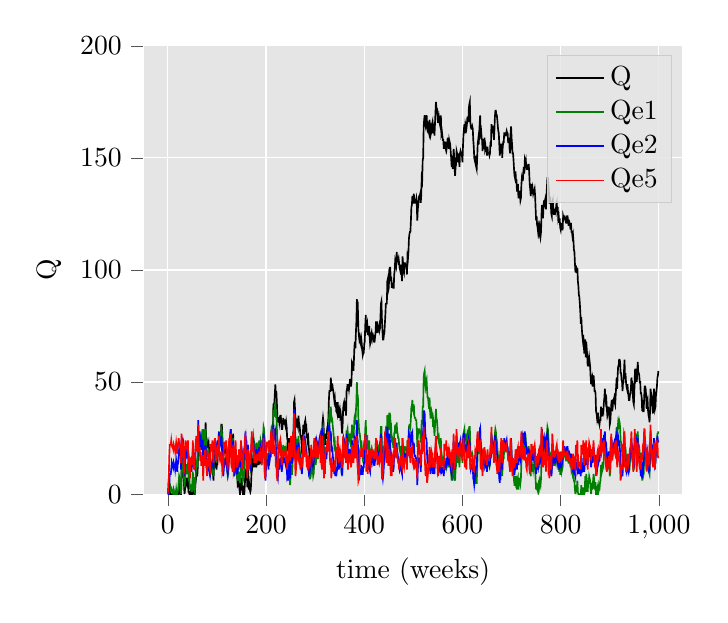
\begin{tikzpicture}

\begin{axis}[
axis background/.style={fill=white!89.8039215686275!black},
axis line style={white},
legend cell align={left},
legend style={fill opacity=0.8, draw opacity=1, text opacity=1, draw=white!80!black, fill=white!89.8039215686275!black},
tick align=outside,
tick pos=left,
x grid style={white},
xlabel={time (weeks)},
xmajorgrids,
xmin=-49.95, xmax=1048.95,
xtick style={color=white!33.3333333333333!black},
y grid style={white},
ylabel={Q},
ymajorgrids,
ymin=0, ymax=200,
ytick style={color=white!33.3333333333333!black}
]
\addplot [semithick, black]
table {%
0 0
1 0
2 0
3 1
4 3
5 0
6 0
7 0
8 0
9 0
10 0
11 0
12 1
13 0
14 0
15 0
16 0
17 1
18 0
19 0
20 0
21 0
22 2
23 4
24 2
25 0
26 0
27 0
28 10
29 12
30 14
31 15
32 8
33 4
34 0
35 2
36 4
37 6
38 7
39 7
40 3
41 7
42 1
43 1
44 0
45 0
46 1
47 0
48 0
49 1
50 0
51 8
52 1
53 1
54 0
55 0
56 4
57 6
58 8
59 10
60 8
61 12
62 22
63 18
64 20
65 24
66 21
67 25
68 22
69 22
70 26
71 29
72 21
73 23
74 23
75 27
76 27
77 32
78 25
79 25
80 21
81 21
82 22
83 23
84 20
85 16
86 13
87 12
88 13
89 12
90 11
91 12
92 9
93 6
94 12
95 12
96 14
97 16
98 15
99 11
100 13
101 15
102 18
103 18
104 24
105 22
106 24
107 26
108 26
109 31
110 31
111 26
112 22
113 17
114 18
115 19
116 20
117 20
118 19
119 21
120 20
121 15
122 11
123 11
124 15
125 20
126 22
127 23
128 29
129 24
130 22
131 22
132 20
133 27
134 18
135 14
136 14
137 13
138 16
139 15
140 11
141 9
142 5
143 6
144 3
145 6
146 2
147 0
148 2
149 7
150 7
151 5
152 2
153 0
154 0
155 2
156 1
157 5
158 11
159 9
160 11
161 9
162 3
163 11
164 9
165 2
166 4
167 2
168 1
169 2
170 7
171 13
172 12
173 14
174 17
175 16
176 12
177 15
178 14
179 14
180 12
181 16
182 14
183 15
184 15
185 13
186 17
187 14
188 14
189 18
190 18
191 13
192 19
193 17
194 22
195 27
196 27
197 23
198 16
199 11
200 14
201 17
202 17
203 17
204 16
205 13
206 16
207 15
208 17
209 17
210 25
211 28
212 27
213 29
214 28
215 40
216 40
217 41
218 45
219 49
220 43
221 46
222 41
223 35
224 32
225 34
226 34
227 32
228 34
229 35
230 35
231 32
232 29
233 29
234 31
235 34
236 31
237 33
238 33
239 31
240 30
241 32
242 30
243 25
244 24
245 19
246 23
247 25
248 19
249 14
250 17
251 21
252 17
253 16
254 19
255 25
256 24
257 41
258 42
259 38
260 32
261 30
262 30
263 32
264 31
265 30
266 35
267 32
268 31
269 29
270 26
271 26
272 24
273 20
274 21
275 27
276 31
277 27
278 27
279 32
280 33
281 31
282 31
283 25
284 27
285 24
286 25
287 21
288 19
289 15
290 14
291 14
292 19
293 17
294 14
295 15
296 11
297 11
298 18
299 18
300 19
301 14
302 16
303 20
304 21
305 17
306 17
307 20
308 21
309 23
310 26
311 24
312 26
313 24
314 22
315 32
316 34
317 32
318 25
319 25
320 22
321 27
322 25
323 25
324 28
325 30
326 31
327 34
328 42
329 46
330 46
331 46
332 52
333 46
334 49
335 49
336 47
337 46
338 44
339 42
340 43
341 39
342 41
343 37
344 37
345 36
346 41
347 37
348 34
349 37
350 38
351 35
352 36
353 34
354 30
355 27
356 31
357 38
358 40
359 41
360 39
361 40
362 39
363 35
364 46
365 47
366 49
367 46
368 49
369 47
370 49
371 51
372 51
373 48
374 50
375 58
376 57
377 58
378 55
379 60
380 66
381 68
382 65
383 72
384 77
385 87
386 82
387 83
388 74
389 71
390 69
391 70
392 68
393 67
394 69
395 67
396 64
397 62
398 63
399 63
400 67
401 68
402 75
403 80
404 74
405 75
406 76
407 71
408 73
409 72
410 75
411 70
412 67
413 68
414 71
415 72
416 70
417 72
418 69
419 71
420 68
421 68
422 70
423 72
424 77
425 74
426 77
427 72
428 74
429 74
430 75
431 73
432 74
433 79
434 85
435 86
436 78
437 73
438 69
439 69
440 71
441 72
442 76
443 80
444 85
445 85
446 85
447 95
448 96
449 91
450 92
451 100
452 101
453 101
454 95
455 97
456 92
457 94
458 94
459 92
460 92
461 98
462 100
463 104
464 103
465 102
466 108
467 105
468 105
469 104
470 105
471 103
472 101
473 100
474 102
475 102
476 98
477 95
478 106
479 103
480 100
481 99
482 103
483 103
484 102
485 102
486 101
487 98
488 106
489 105
490 108
491 114
492 116
493 117
494 117
495 122
496 128
497 129
498 133
499 130
500 130
501 134
502 130
503 130
504 131
505 131
506 132
507 129
508 122
509 127
510 129
511 132
512 133
513 133
514 134
515 130
516 133
517 141
518 140
519 149
520 150
521 164
522 167
523 169
524 165
525 164
526 167
527 169
528 165
529 163
530 164
531 162
532 161
533 167
534 162
535 160
536 161
537 165
538 165
539 166
540 161
541 164
542 163
543 160
544 165
545 170
546 175
547 172
548 172
549 170
550 166
551 166
552 168
553 166
554 165
555 164
556 169
557 161
558 162
559 160
560 158
561 158
562 154
563 157
564 157
565 155
566 154
567 157
568 155
569 157
570 159
571 156
572 154
573 158
574 157
575 156
576 153
577 150
578 146
579 151
580 145
581 148
582 154
583 151
584 145
585 142
586 146
587 147
588 153
589 152
590 148
591 150
592 152
593 149
594 146
595 152
596 153
597 152
598 152
599 151
600 148
601 155
602 160
603 163
604 165
605 161
606 165
607 164
608 163
609 165
610 168
611 168
612 166
613 172
614 174
615 175
616 166
617 164
618 163
619 163
620 164
621 163
622 158
623 155
624 150
625 149
626 151
627 147
628 146
629 145
630 150
631 156
632 158
633 156
634 161
635 165
636 169
637 161
638 162
639 159
640 158
641 153
642 158
643 158
644 154
645 159
646 154
647 155
648 153
649 153
650 151
651 155
652 152
653 152
654 152
655 151
656 152
657 157
658 155
659 165
660 161
661 164
662 164
663 164
664 158
665 162
666 168
667 171
668 171
669 169
670 169
671 167
672 164
673 162
674 161
675 156
676 151
677 154
678 152
679 156
680 156
681 150
682 155
683 157
684 157
685 161
686 161
687 160
688 160
689 161
690 162
691 161
692 161
693 157
694 157
695 159
696 154
697 152
698 161
699 164
700 159
701 156
702 152
703 152
704 149
705 145
706 142
707 141
708 144
709 140
710 140
711 135
712 138
713 138
714 132
715 135
716 135
717 134
718 131
719 132
720 138
721 141
722 140
723 140
724 144
725 146
726 143
727 149
728 148
729 149
730 146
731 145
732 145
733 145
734 147
735 147
736 143
737 138
738 136
739 133
740 138
741 138
742 134
743 136
744 134
745 135
746 135
747 136
748 133
749 127
750 122
751 124
752 120
753 119
754 117
755 119
756 117
757 119
758 117
759 115
760 117
761 125
762 129
763 126
764 123
765 128
766 131
767 128
768 131
769 132
770 127
771 133
772 137
773 141
774 141
775 138
776 135
777 130
778 130
779 131
780 129
781 125
782 124
783 130
784 131
785 127
786 125
787 125
788 127
789 127
790 126
791 129
792 130
793 126
794 128
795 123
796 124
797 121
798 123
799 119
800 118
801 121
802 118
803 118
804 118
805 124
806 123
807 124
808 124
809 123
810 122
811 121
812 121
813 124
814 124
815 122
816 120
817 120
818 121
819 120
820 118
821 121
822 117
823 117
824 115
825 116
826 113
827 109
828 108
829 103
830 99
831 102
832 99
833 99
834 101
835 95
836 93
837 89
838 88
839 85
840 81
841 76
842 79
843 74
844 71
845 69
846 71
847 67
848 63
849 63
850 69
851 61
852 68
853 65
854 62
855 57
856 60
857 59
858 61
859 59
860 57
861 52
862 49
863 51
864 52
865 48
866 51
867 53
868 50
869 46
870 46
871 45
872 37
873 36
874 34
875 36
876 36
877 32
878 32
879 31
880 33
881 33
882 39
883 35
884 35
885 38
886 38
887 37
888 41
889 43
890 47
891 43
892 41
893 42
894 38
895 35
896 36
897 36
898 39
899 37
900 31
901 32
902 36
903 40
904 42
905 37
906 39
907 42
908 42
909 43
910 41
911 40
912 44
913 48
914 52
915 47
916 53
917 57
918 57
919 60
920 60
921 59
922 54
923 54
924 51
925 50
926 46
927 50
928 50
929 55
930 60
931 52
932 54
933 50
934 48
935 47
936 49
937 46
938 44
939 42
940 42
941 44
942 45
943 47
944 52
945 50
946 50
947 44
948 41
949 40
950 46
951 53
952 52
953 56
954 53
955 50
956 55
957 59
958 54
959 54
960 53
961 50
962 50
963 45
964 45
965 43
966 37
967 39
968 37
969 37
970 43
971 48
972 48
973 47
974 44
975 38
976 41
977 42
978 37
979 35
980 34
981 32
982 37
983 47
984 45
985 44
986 41
987 38
988 36
989 43
990 47
991 44
992 38
993 39
994 44
995 46
996 48
997 52
998 53
999 55
};
\addlegendentry{Q}
\addplot [semithick, green!50.1960784313725!black]
table {%
0 0
1 0
2 0
3 2
4 5
5 3
6 1
7 1
8 2
9 1
10 1
11 0
12 2
13 1
14 1
15 0
16 0
17 2
18 0
19 0
20 1
21 2
22 5
23 8
24 7
25 6
26 5
27 0
28 11
29 14
30 16
31 17
32 10
33 7
34 3
35 6
36 9
37 12
38 13
39 13
40 9
41 14
42 8
43 9
44 7
45 2
46 4
47 4
48 1
49 3
50 1
51 10
52 4
53 5
54 2
55 1
56 6
57 9
58 12
59 14
60 12
61 16
62 26
63 21
64 23
65 27
66 23
67 27
68 23
69 23
70 27
71 29
72 20
73 22
74 22
75 26
76 25
77 29
78 21
79 21
80 17
81 17
82 18
83 19
84 16
85 12
86 9
87 9
88 11
89 11
90 11
91 13
92 10
93 8
94 15
95 15
96 17
97 19
98 18
99 14
100 16
101 18
102 21
103 21
104 27
105 24
106 25
107 26
108 25
109 29
110 28
111 22
112 18
113 13
114 14
115 15
116 16
117 16
118 15
119 17
120 16
121 11
122 8
123 9
124 14
125 19
126 21
127 22
128 28
129 22
130 20
131 20
132 18
133 25
134 15
135 11
136 12
137 11
138 15
139 14
140 10
141 9
142 6
143 8
144 6
145 10
146 7
147 5
148 8
149 14
150 14
151 12
152 9
153 6
154 7
155 10
156 10
157 15
158 21
159 19
160 21
161 19
162 13
163 21
164 19
165 12
166 14
167 12
168 11
169 13
170 18
171 24
172 22
173 24
174 26
175 24
176 19
177 22
178 21
179 21
180 19
181 23
182 21
183 22
184 22
185 20
186 24
187 20
188 20
189 24
190 23
191 18
192 24
193 21
194 26
195 30
196 29
197 24
198 16
199 11
200 15
201 18
202 18
203 18
204 17
205 14
206 17
207 16
208 18
209 18
210 26
211 28
212 26
213 27
214 25
215 36
216 35
217 35
218 38
219 41
220 34
221 36
222 30
223 23
224 20
225 22
226 22
227 20
228 22
229 23
230 23
231 20
232 17
233 17
234 19
235 22
236 19
237 21
238 21
239 19
240 18
241 20
242 18
243 13
244 12
245 7
246 12
247 14
248 8
249 4
250 8
251 13
252 9
253 9
254 13
255 19
256 18
257 35
258 35
259 30
260 23
261 21
262 21
263 23
264 22
265 21
266 26
267 22
268 21
269 19
270 16
271 16
272 14
273 10
274 12
275 18
276 22
277 18
278 18
279 23
280 24
281 21
282 21
283 15
284 17
285 14
286 15
287 11
288 10
289 7
290 7
291 8
292 14
293 12
294 9
295 11
296 8
297 9
298 17
299 17
300 18
301 13
302 15
303 19
304 20
305 16
306 16
307 19
308 20
309 22
310 25
311 22
312 24
313 21
314 19
315 29
316 30
317 27
318 19
319 19
320 16
321 21
322 19
323 19
324 22
325 24
326 24
327 26
328 33
329 36
330 35
331 34
332 39
333 32
334 34
335 33
336 30
337 28
338 25
339 22
340 23
341 19
342 21
343 17
344 17
345 16
346 21
347 17
348 14
349 17
350 18
351 15
352 16
353 14
354 10
355 8
356 13
357 20
358 22
359 23
360 21
361 22
362 21
363 17
364 28
365 28
366 29
367 25
368 27
369 24
370 25
371 26
372 25
373 21
374 23
375 31
376 29
377 29
378 25
379 29
380 34
381 35
382 31
383 37
384 41
385 50
386 44
387 44
388 34
389 30
390 27
391 27
392 24
393 22
394 24
395 21
396 18
397 16
398 17
399 17
400 21
401 22
402 29
403 33
404 26
405 26
406 26
407 20
408 22
409 21
410 24
411 18
412 15
413 16
414 19
415 20
416 18
417 20
418 17
419 19
420 16
421 16
422 18
423 20
424 25
425 21
426 24
427 18
428 20
429 20
430 21
431 19
432 20
433 25
434 30
435 30
436 21
437 16
438 12
439 12
440 14
441 15
442 19
443 23
444 28
445 27
446 26
447 35
448 35
449 29
450 29
451 36
452 36
453 35
454 28
455 29
456 23
457 25
458 24
459 21
460 21
461 27
462 28
463 31
464 29
465 27
466 32
467 28
468 27
469 25
470 25
471 22
472 20
473 19
474 21
475 21
476 17
477 14
478 25
479 21
480 18
481 17
482 21
483 21
484 20
485 20
486 19
487 16
488 24
489 22
490 25
491 30
492 31
493 31
494 30
495 34
496 39
497 39
498 42
499 38
500 37
501 40
502 35
503 34
504 34
505 33
506 33
507 29
508 21
509 26
510 27
511 29
512 29
513 28
514 28
515 23
516 26
517 33
518 31
519 39
520 39
521 52
522 54
523 55
524 50
525 48
526 50
527 51
528 46
529 43
530 43
531 40
532 38
533 43
534 37
535 34
536 34
537 37
538 36
539 36
540 30
541 32
542 30
543 26
544 30
545 34
546 38
547 34
548 33
549 30
550 25
551 24
552 25
553 22
554 21
555 20
556 25
557 16
558 17
559 15
560 13
561 13
562 9
563 13
564 13
565 11
566 11
567 15
568 13
569 15
570 17
571 14
572 12
573 16
574 15
575 14
576 11
577 9
578 6
579 12
580 6
581 10
582 17
583 14
584 8
585 6
586 11
587 13
588 19
589 18
590 14
591 16
592 18
593 15
594 12
595 18
596 19
597 18
598 18
599 17
600 14
601 21
602 26
603 28
604 29
605 24
606 27
607 25
608 23
609 25
610 27
611 26
612 23
613 29
614 30
615 30
616 20
617 18
618 17
619 17
620 18
621 17
622 12
623 9
624 5
625 5
626 8
627 5
628 5
629 5
630 11
631 18
632 20
633 18
634 23
635 27
636 30
637 21
638 22
639 19
640 18
641 13
642 18
643 18
644 14
645 19
646 14
647 15
648 13
649 13
650 11
651 16
652 13
653 13
654 13
655 12
656 13
657 18
658 16
659 26
660 21
661 24
662 23
663 23
664 17
665 21
666 27
667 29
668 28
669 25
670 24
671 21
672 18
673 16
674 15
675 10
676 6
677 10
678 9
679 14
680 14
681 8
682 14
683 16
684 16
685 20
686 20
687 19
688 19
689 20
690 21
691 20
692 20
693 16
694 16
695 18
696 13
697 11
698 21
699 24
700 18
701 15
702 11
703 12
704 9
705 6
706 4
707 4
708 8
709 5
710 6
711 2
712 6
713 7
714 2
715 6
716 7
717 7
718 5
719 7
720 14
721 17
722 16
723 16
724 20
725 22
726 19
727 25
728 23
729 24
730 20
731 19
732 19
733 19
734 21
735 21
736 17
737 12
738 10
739 8
740 14
741 14
742 10
743 13
744 11
745 13
746 13
747 14
748 11
749 6
750 2
751 5
752 2
753 2
754 1
755 4
756 3
757 6
758 5
759 4
760 7
761 16
762 20
763 17
764 14
765 19
766 22
767 19
768 22
769 23
770 18
771 24
772 27
773 30
774 29
775 25
776 21
777 16
778 16
779 17
780 15
781 11
782 11
783 18
784 19
785 15
786 13
787 13
788 15
789 15
790 14
791 17
792 18
793 14
794 16
795 11
796 13
797 10
798 13
799 9
800 9
801 13
802 10
803 11
804 12
805 18
806 17
807 18
808 18
809 17
810 16
811 15
812 15
813 18
814 18
815 16
816 14
817 14
818 15
819 14
820 12
821 15
822 11
823 12
824 10
825 12
826 9
827 6
828 6
829 2
830 0
831 4
832 2
833 3
834 6
835 1
836 0
837 0
838 0
839 0
840 0
841 0
842 4
843 0
844 0
845 0
846 3
847 0
848 0
849 1
850 8
851 1
852 9
853 7
854 5
855 1
856 5
857 5
858 8
859 7
860 6
861 2
862 0
863 3
864 5
865 2
866 6
867 9
868 7
869 4
870 5
871 5
872 0
873 0
874 0
875 3
876 4
877 1
878 2
879 2
880 5
881 6
882 13
883 9
884 10
885 14
886 14
887 13
888 17
889 19
890 23
891 19
892 17
893 18
894 14
895 11
896 13
897 13
898 16
899 14
900 8
901 10
902 15
903 19
904 21
905 16
906 18
907 21
908 21
909 22
910 20
911 19
912 23
913 27
914 30
915 24
916 29
917 32
918 31
919 33
920 32
921 30
922 24
923 23
924 20
925 19
926 15
927 19
928 19
929 24
930 28
931 19
932 21
933 17
934 15
935 14
936 16
937 13
938 11
939 10
940 11
941 14
942 15
943 17
944 22
945 20
946 20
947 14
948 11
949 11
950 18
951 25
952 23
953 27
954 23
955 20
956 25
957 28
958 22
959 22
960 21
961 18
962 18
963 13
964 13
965 11
966 6
967 9
968 8
969 9
970 16
971 21
972 21
973 20
974 17
975 11
976 15
977 16
978 11
979 10
980 10
981 9
982 15
983 25
984 22
985 21
986 18
987 15
988 13
989 20
990 24
991 20
992 14
993 15
994 20
995 22
996 24
997 27
998 27
999 28
};
\addlegendentry{Qe1}
\addplot [semithick, blue]
table {%
0 0
1 0
2 0
3 4
4 9
5 9
6 9
7 11
8 14
9 13
10 13
11 12
12 14
13 13
14 13
15 11
16 13
17 15
18 13
19 10
20 13
21 14
22 17
23 20
24 19
25 18
26 17
27 11
28 24
29 25
30 25
31 24
32 15
33 12
34 8
35 13
36 16
37 19
38 20
39 20
40 16
41 21
42 15
43 16
44 14
45 9
46 13
47 13
48 10
49 14
50 12
51 21
52 15
53 16
54 13
55 12
56 17
57 20
58 23
59 25
60 21
61 25
62 33
63 26
64 26
65 28
66 22
67 26
68 20
69 20
70 24
71 24
72 13
73 15
74 15
75 19
76 18
77 22
78 14
79 14
80 10
81 12
82 13
83 14
84 11
85 9
86 8
87 10
88 14
89 14
90 14
91 16
92 13
93 11
94 20
95 20
96 22
97 24
98 21
99 17
100 19
101 21
102 24
103 22
104 28
105 23
106 24
107 23
108 22
109 26
110 23
111 17
112 13
113 8
114 11
115 14
116 15
117 15
118 14
119 16
120 15
121 10
122 9
123 12
124 17
125 22
126 24
127 23
128 29
129 21
130 19
131 19
132 17
133 24
134 12
135 8
136 11
137 12
138 16
139 15
140 11
141 12
142 9
143 13
144 11
145 17
146 14
147 12
148 15
149 21
150 21
151 19
152 16
153 13
154 14
155 17
156 17
157 22
158 28
159 24
160 24
161 20
162 14
163 22
164 20
165 13
166 15
167 13
168 12
169 14
170 19
171 25
172 21
173 23
174 25
175 21
176 16
177 19
178 18
179 18
180 16
181 20
182 18
183 19
184 19
185 17
186 21
187 17
188 17
189 21
190 20
191 15
192 21
193 18
194 23
195 27
196 24
197 17
198 9
199 6
200 12
201 15
202 15
203 15
204 14
205 11
206 16
207 15
208 17
209 17
210 25
211 25
212 21
213 22
214 20
215 31
216 28
217 26
218 27
219 28
220 19
221 21
222 15
223 8
224 7
225 11
226 13
227 11
228 15
229 16
230 16
231 13
232 10
233 12
234 14
235 17
236 14
237 16
238 16
239 14
240 13
241 15
242 13
243 8
244 9
245 6
246 13
247 15
248 9
249 7
250 13
251 18
252 14
253 14
254 18
255 24
256 21
257 38
258 36
259 29
260 20
261 18
262 18
263 20
264 19
265 18
266 23
267 19
268 18
269 16
270 13
271 13
272 11
273 9
274 13
275 19
276 23
277 19
278 19
279 24
280 23
281 20
282 20
283 14
284 16
285 13
286 14
287 10
288 11
289 10
290 12
291 13
292 19
293 17
294 14
295 16
296 13
297 14
298 22
299 22
300 23
301 18
302 20
303 24
304 23
305 19
306 19
307 22
308 23
309 25
310 26
311 21
312 23
313 20
314 18
315 28
316 27
317 22
318 14
319 14
320 11
321 18
322 16
323 16
324 19
325 21
326 21
327 23
328 30
329 31
330 28
331 25
332 28
333 19
334 21
335 20
336 17
337 15
338 12
339 9
340 12
341 8
342 12
343 8
344 10
345 11
346 18
347 14
348 11
349 16
350 17
351 14
352 15
353 13
354 9
355 9
356 16
357 23
358 25
359 24
360 20
361 21
362 20
363 16
364 27
365 25
366 24
367 18
368 20
369 17
370 18
371 19
372 18
373 14
374 16
375 24
376 20
377 20
378 16
379 20
380 25
381 24
382 18
383 24
384 26
385 33
386 25
387 23
388 13
389 9
390 8
391 10
392 9
393 9
394 13
395 10
396 9
397 9
398 12
399 12
400 16
401 17
402 24
403 26
404 17
405 17
406 17
407 11
408 15
409 14
410 17
411 11
412 10
413 13
414 16
415 17
416 15
417 17
418 14
419 16
420 13
421 13
422 15
423 17
424 22
425 18
426 21
427 15
428 17
429 17
430 18
431 16
432 17
433 22
434 27
435 25
436 14
437 9
438 7
439 9
440 13
441 14
442 18
443 22
444 27
445 24
446 21
447 30
448 28
449 20
450 20
451 27
452 25
453 22
454 15
455 16
456 10
457 14
458 13
459 10
460 12
461 18
462 19
463 22
464 20
465 18
466 23
467 19
468 18
469 16
470 16
471 13
472 11
473 12
474 14
475 14
476 10
477 9
478 22
479 18
480 15
481 14
482 18
483 18
484 17
485 17
486 16
487 13
488 21
489 19
490 22
491 27
492 26
493 24
494 21
495 25
496 28
497 26
498 27
499 21
500 20
501 23
502 18
503 17
504 17
505 16
506 16
507 12
508 4
509 11
510 14
511 16
512 16
513 15
514 15
515 10
516 15
517 22
518 20
519 28
520 26
521 37
522 37
523 36
524 29
525 25
526 25
527 24
528 17
529 14
530 14
531 11
532 11
533 18
534 12
535 9
536 11
537 16
538 15
539 15
540 9
541 13
542 11
543 9
544 15
545 19
546 23
547 19
548 18
549 15
550 10
551 11
552 14
553 11
554 12
555 11
556 18
557 9
558 12
559 10
560 10
561 12
562 8
563 14
564 14
565 12
566 12
567 16
568 14
569 16
570 18
571 15
572 13
573 17
574 16
575 15
576 12
577 10
578 9
579 17
580 11
581 17
582 24
583 19
584 13
585 11
586 18
587 20
588 26
589 23
590 19
591 21
592 23
593 20
594 17
595 23
596 24
597 21
598 21
599 20
600 17
601 24
602 27
603 27
604 26
605 19
606 22
607 20
608 18
609 20
610 22
611 21
612 18
613 24
614 23
615 23
616 13
617 11
618 12
619 12
620 13
621 12
622 7
623 6
624 4
625 6
626 11
627 10
628 12
629 12
630 18
631 25
632 25
633 21
634 26
635 28
636 29
637 18
638 19
639 16
640 15
641 10
642 17
643 17
644 13
645 18
646 13
647 14
648 12
649 12
650 10
651 17
652 14
653 14
654 14
655 13
656 14
657 19
658 17
659 27
660 20
661 23
662 22
663 22
664 16
665 20
666 26
667 26
668 23
669 20
670 19
671 16
672 13
673 11
674 12
675 7
676 5
677 11
678 12
679 17
680 17
681 11
682 19
683 21
684 21
685 25
686 23
687 22
688 22
689 23
690 24
691 21
692 21
693 17
694 17
695 19
696 14
697 12
698 22
699 25
700 17
701 14
702 10
703 13
704 10
705 9
706 9
707 11
708 17
709 14
710 15
711 11
712 17
713 18
714 13
715 17
716 18
717 18
718 16
719 18
720 25
721 26
722 23
723 23
724 27
725 27
726 22
727 28
728 24
729 23
730 19
731 18
732 18
733 18
734 20
735 20
736 16
737 11
738 11
739 11
740 19
741 19
742 15
743 18
744 16
745 18
746 18
747 19
748 16
749 11
750 9
751 14
752 11
753 13
754 12
755 15
756 14
757 17
758 16
759 15
760 18
761 27
762 29
763 24
764 19
765 24
766 25
767 20
768 23
769 24
770 17
771 23
772 26
773 27
774 24
775 18
776 14
777 9
778 11
779 14
780 12
781 8
782 10
783 19
784 20
785 16
786 14
787 14
788 16
789 16
790 15
791 18
792 19
793 15
794 17
795 12
796 14
797 11
798 16
799 12
800 12
801 16
802 13
803 14
804 15
805 21
806 20
807 21
808 21
809 20
810 19
811 18
812 18
813 21
814 21
815 19
816 17
817 17
818 18
819 17
820 15
821 18
822 14
823 15
824 13
825 15
826 12
827 9
828 11
829 9
830 8
831 14
832 12
833 13
834 16
835 11
836 12
837 9
838 11
839 11
840 10
841 8
842 14
843 10
844 10
845 11
846 16
847 13
848 10
849 13
850 20
851 13
852 21
853 19
854 17
855 13
856 17
857 17
858 20
859 19
860 18
861 14
862 12
863 15
864 17
865 14
866 18
867 21
868 19
869 16
870 17
871 17
872 10
873 12
874 11
875 16
876 17
877 14
878 15
879 15
880 18
881 19
882 26
883 20
884 21
885 25
886 23
887 22
888 26
889 26
890 28
891 22
892 20
893 21
894 17
895 14
896 16
897 16
898 19
899 17
900 11
901 15
902 20
903 24
904 24
905 17
906 19
907 22
908 22
909 23
910 21
911 20
912 24
913 26
914 27
915 19
916 24
917 25
918 22
919 24
920 21
921 19
922 13
923 12
924 9
925 10
926 8
927 14
928 14
929 19
930 23
931 14
932 16
933 12
934 10
935 11
936 15
937 12
938 10
939 11
940 14
941 17
942 18
943 20
944 25
945 21
946 21
947 15
948 12
949 12
950 19
951 26
952 22
953 26
954 20
955 17
956 22
957 25
958 17
959 17
960 16
961 13
962 13
963 8
964 10
965 10
966 7
967 12
968 11
969 14
970 21
971 26
972 24
973 21
974 18
975 12
976 16
977 17
978 12
979 11
980 13
981 12
982 18
983 28
984 23
985 22
986 19
987 16
988 14
989 21
990 25
991 19
992 13
993 14
994 19
995 21
996 23
997 26
998 24
999 23
};
\addlegendentry{Qe2}
\addplot [semithick, red]
table {%
0 0
1 5
2 8
3 17
4 22
5 22
6 22
7 24
8 22
9 21
10 21
11 20
12 22
13 21
14 21
15 19
16 21
17 23
18 21
19 18
20 21
21 22
22 25
23 23
24 22
25 21
26 20
27 14
28 27
29 23
30 23
31 22
32 13
33 10
34 11
35 21
36 24
37 22
38 23
39 23
40 19
41 24
42 13
43 14
44 12
45 7
46 16
47 16
48 13
49 17
50 15
51 24
52 13
53 14
54 11
55 15
56 20
57 23
58 26
59 23
60 19
61 23
62 31
63 19
64 19
65 21
66 15
67 19
68 13
69 13
70 17
71 17
72 6
73 13
74 13
75 17
76 16
77 20
78 12
79 12
80 8
81 15
82 16
83 17
84 14
85 12
86 11
87 18
88 22
89 22
90 22
91 24
92 16
93 14
94 23
95 23
96 25
97 22
98 19
99 15
100 17
101 19
102 22
103 20
104 26
105 16
106 17
107 16
108 15
109 19
110 16
111 10
112 11
113 11
114 19
115 22
116 23
117 23
118 22
119 24
120 18
121 13
122 12
123 15
124 20
125 25
126 22
127 21
128 27
129 14
130 12
131 12
132 10
133 22
134 10
135 11
136 19
137 20
138 24
139 18
140 14
141 15
142 12
143 16
144 14
145 20
146 17
147 15
148 18
149 24
150 19
151 17
152 14
153 11
154 17
155 20
156 20
157 25
158 26
159 17
160 17
161 13
162 7
163 20
164 18
165 11
166 18
167 16
168 15
169 17
170 22
171 28
172 19
173 21
174 23
175 19
176 14
177 17
178 16
179 16
180 14
181 18
182 16
183 17
184 17
185 15
186 19
187 15
188 15
189 19
190 18
191 13
192 19
193 16
194 21
195 25
196 17
197 10
198 7
199 9
200 20
201 23
202 23
203 23
204 22
205 19
206 24
207 18
208 20
209 20
210 28
211 23
212 19
213 20
214 18
215 29
216 21
217 19
218 20
219 21
220 12
221 14
222 8
223 6
224 10
225 19
226 21
227 19
228 23
229 24
230 19
231 16
232 13
233 15
234 17
235 20
236 17
237 19
238 19
239 17
240 16
241 18
242 16
243 11
244 17
245 14
246 21
247 23
248 17
249 15
250 21
251 26
252 17
253 17
254 21
255 27
256 19
257 36
258 29
259 17
260 8
261 11
262 16
263 18
264 17
265 16
266 21
267 17
268 16
269 14
270 11
271 16
272 14
273 12
274 16
275 22
276 26
277 17
278 17
279 22
280 21
281 18
282 18
283 12
284 14
285 11
286 17
287 13
288 14
289 13
290 15
291 16
292 22
293 20
294 17
295 19
296 16
297 17
298 25
299 20
300 21
301 16
302 18
303 22
304 21
305 17
306 17
307 20
308 21
309 23
310 24
311 14
312 16
313 13
314 11
315 26
316 20
317 15
318 7
319 12
320 9
321 21
322 19
323 19
324 22
325 24
326 19
327 21
328 28
329 24
330 16
331 13
332 16
333 7
334 14
335 13
336 10
337 13
338 10
339 12
340 15
341 11
342 20
343 16
344 18
345 19
346 26
347 17
348 14
349 19
350 20
351 17
352 18
353 16
354 12
355 12
356 19
357 26
358 23
359 22
360 18
361 19
362 18
363 14
364 25
365 18
366 17
367 11
368 18
369 15
370 16
371 17
372 16
373 12
374 14
375 22
376 18
377 18
378 14
379 18
380 23
381 22
382 16
383 22
384 24
385 26
386 13
387 11
388 6
389 7
390 11
391 18
392 17
393 17
394 21
395 18
396 17
397 17
398 20
399 20
400 24
401 20
402 27
403 24
404 10
405 15
406 15
407 9
408 18
409 17
410 20
411 14
412 13
413 16
414 19
415 20
416 18
417 20
418 17
419 19
420 16
421 16
422 18
423 20
424 25
425 16
426 19
427 13
428 15
429 15
430 16
431 14
432 15
433 20
434 25
435 18
436 7
437 7
438 10
439 17
440 21
441 22
442 26
443 25
444 25
445 17
446 14
447 23
448 21
449 13
450 13
451 20
452 18
453 15
454 8
455 14
456 8
457 17
458 16
459 13
460 15
461 21
462 22
463 25
464 18
465 16
466 21
467 17
468 16
469 14
470 14
471 11
472 14
473 15
474 17
475 17
476 13
477 12
478 25
479 16
480 13
481 12
482 16
483 16
484 15
485 15
486 14
487 11
488 24
489 17
490 20
491 25
492 19
493 17
494 14
495 18
496 21
497 19
498 20
499 14
500 13
501 16
502 11
503 15
504 15
505 14
506 14
507 10
508 7
509 19
510 22
511 24
512 19
513 18
514 18
515 13
516 18
517 25
518 18
519 26
520 19
521 30
522 25
523 19
524 12
525 8
526 13
527 12
528 5
529 7
530 12
531 9
532 14
533 21
534 15
535 12
536 14
537 19
538 18
539 18
540 12
541 16
542 14
543 12
544 18
545 22
546 26
547 17
548 16
549 13
550 8
551 14
552 17
553 14
554 15
555 14
556 21
557 12
558 15
559 13
560 13
561 15
562 11
563 22
564 22
565 20
566 20
567 24
568 17
569 19
570 21
571 18
572 16
573 20
574 19
575 18
576 15
577 13
578 12
579 20
580 14
581 20
582 27
583 17
584 11
585 14
586 21
587 23
588 29
589 21
590 17
591 19
592 21
593 18
594 15
595 21
596 22
597 19
598 19
599 18
600 15
601 22
602 25
603 20
604 19
605 12
606 15
607 13
608 11
609 18
610 20
611 19
612 16
613 22
614 21
615 21
616 11
617 14
618 15
619 15
620 16
621 15
622 10
623 14
624 12
625 14
626 19
627 18
628 20
629 20
630 26
631 28
632 23
633 19
634 24
635 21
636 22
637 11
638 17
639 14
640 13
641 8
642 20
643 20
644 16
645 21
646 16
647 17
648 15
649 15
650 13
651 20
652 17
653 17
654 17
655 16
656 17
657 22
658 20
659 30
660 18
661 21
662 20
663 20
664 14
665 18
666 24
667 19
668 16
669 13
670 12
671 9
672 11
673 14
674 15
675 10
676 13
677 19
678 20
679 25
680 20
681 14
682 22
683 24
684 19
685 23
686 21
687 20
688 20
689 21
690 22
691 19
692 19
693 15
694 15
695 17
696 12
697 10
698 25
699 23
700 15
701 12
702 8
703 16
704 13
705 12
706 12
707 14
708 20
709 17
710 18
711 14
712 20
713 21
714 16
715 20
716 21
717 21
718 19
719 21
720 28
721 24
722 16
723 16
724 20
725 20
726 15
727 21
728 17
729 16
730 12
731 11
732 16
733 16
734 18
735 18
736 14
737 9
738 14
739 14
740 22
741 22
742 18
743 21
744 19
745 21
746 21
747 22
748 19
749 14
750 12
751 17
752 14
753 16
754 15
755 18
756 17
757 20
758 19
759 18
760 21
761 30
762 27
763 17
764 12
765 17
766 18
767 13
768 16
769 17
770 10
771 21
772 24
773 20
774 17
775 11
776 12
777 7
778 14
779 17
780 15
781 11
782 18
783 27
784 23
785 19
786 17
787 17
788 19
789 19
790 18
791 21
792 22
793 18
794 20
795 15
796 17
797 14
798 19
799 15
800 15
801 19
802 16
803 17
804 18
805 24
806 18
807 19
808 19
809 18
810 17
811 16
812 16
813 19
814 19
815 17
816 15
817 15
818 16
819 15
820 13
821 16
822 12
823 13
824 11
825 18
826 15
827 12
828 14
829 12
830 11
831 22
832 20
833 21
834 24
835 14
836 15
837 12
838 14
839 14
840 13
841 11
842 22
843 18
844 18
845 19
846 24
847 16
848 13
849 16
850 23
851 16
852 24
853 17
854 15
855 11
856 20
857 20
858 23
859 22
860 21
861 17
862 15
863 18
864 20
865 17
866 21
867 24
868 17
869 14
870 15
871 15
872 8
873 15
874 14
875 19
876 20
877 17
878 18
879 18
880 21
881 22
882 29
883 18
884 19
885 23
886 21
887 20
888 24
889 19
890 21
891 15
892 13
893 14
894 10
895 12
896 14
897 14
898 17
899 15
900 9
901 18
902 23
903 27
904 22
905 15
906 17
907 20
908 20
909 21
910 19
911 18
912 22
913 24
914 20
915 12
916 17
917 18
918 15
919 17
920 14
921 12
922 6
923 10
924 12
925 13
926 11
927 22
928 22
929 27
930 26
931 12
932 14
933 10
934 13
935 14
936 18
937 15
938 13
939 14
940 17
941 20
942 21
943 23
944 28
945 19
946 19
947 13
948 10
949 15
950 22
951 29
952 20
953 24
954 13
955 10
956 20
957 23
958 15
959 15
960 14
961 11
962 16
963 11
964 18
965 18
966 15
967 20
968 19
969 22
970 29
971 29
972 22
973 19
974 16
975 10
976 19
977 20
978 15
979 14
980 16
981 15
982 21
983 31
984 21
985 20
986 17
987 14
988 12
989 19
990 23
991 17
992 11
993 17
994 22
995 24
996 21
997 24
998 17
999 16
};
\addlegendentry{Qe5}
\end{axis}

\end{tikzpicture}
  
\caption{Controlling the number of intakes. Clearly, adapting the
  service rate `does wonders' to control the queue length.}
\label{fig:intakes}
\end{figure}


From this simulation experiment, we learn that changing holiday plans or spreading the work over multiple servers, i.e., psychiatrists, does not significantly affect the queueing behavior.
However, controlling the service rate as a function of the queue length improves the situation quite dramatically.


\subsection*{Conclusion}
\label{sec:conclusion}

From the above case we learn that even with these (deceitfully) simple recursions, we can obtain considerable insight into the behavior and performance of this quite complicated controlled queueing system\footnote{If you doubt the value of simulation, try to develop a mathematical method to analyze multi-server queueing systems with vacations, of which this case is an example.}.
In general, the study of queueing systems is focused on studying the probabilistic properties of the queueing length process and related concepts such as waiting time, server occupancy, fraction of customers lost, and so on.
Once we have constructed the queueing process, we can compute all relevant performance measures, such as the average waiting time.
If it turns out that the performance of the system is not according to what we desire, we can change parts of the system with the aim to improve the situation and assess the effect of this change.
For instance, if the average waiting time is too long, we might want to add service capacity.
With simulation it is easy to study, hence evaluate, the effect of such decisions.

\subsection*{Exercises}
\label{sec:exercises-1}


The reader should understand from the above case that, once we have the recursions, we can analyze the system and make, for instance, plots to evaluate suggestions for improvement.
Thus, formulating the recursions is crucial to construct queueing processes.
For this reason, many  of the exercises below concentrate on obtaining recursions for specific queueing systems.

It may be that the recursions you find are not identical to the recursions in the solution.
The reason is that the assumptions you make might not be equal to the ones I make.
I don't quite know how to get out of this paradoxical situation.
In a sense, to completely specify the model, we need the recursions.
However, if the problem statement would contain the recursions, there would be nothing left to practice anymore.
Another way is to make the problem description five times as long, but this is also undesirable.
So, let's be pragmatic: the aim is that you practice with modeling, and that you learn from the solutions.
If you obtain \emph{reasonable} recursions, but they are different from mine, then your answer is just as good.

\begin{exercise}[Queue with Blocking]\clabel{ex:l-115} 
A queueing system
  under daily review, i.e., at the end of the day the queue length is
  measured. We assume that at the end of the day no jobs are still in
  service. We assume that jobs that arrive at day $k$ cannot be served
  in day $k$. The queue length cannot exceed level $K$.  Formulate a
  set of recursions to cover this case. What is the loss per period? What is the fraction of jobs lost?
\begin{solution}
  All jobs that arrive such that the queue becomes larger than $K$ must be dropped.

First $d_k = \min\{L_{k-1}, c_k\}$. Then, $L_k' = L_{k-1}+a_k-d_k$ is the queue without blocking. Then $L_k=\min\{L_k', K\}$ is the queue with blocking. Finally, the loss $l_k=L_k'-L_k$, i.e., the excess arrivals. The fraction lost is $l_k/a_k$. 
\end{solution}
\end{exercise}

\begin{exercise}[Estimating the lead time distribution] \clabel{ex:19} 
Take $d_k = \min\{L_{k-1}+a_k, c_k\}$, and assume that jobs are served in FIFO sequence.
  Find an expression for the shortest possible waiting time $W_{-,k}$ of a job that arrives at time $k$, and an expression for the largest possible waiting time $W_{+,k}$.
\begin{hint}
  Consider a numerical example.
  Suppose $L_{k-1}=20$.
  Suppose that the capacity is $c_k=3$ for all $k$.
  Then a job that arrives in the $k$th period, must wait at least $20/3$ (plus rounding) periods before it can leave the system.
  Now generalize this numerical example.
\end{hint}
\begin{solution}
  Let's tag the first customer that arrives in period $k$.
  This tagged customer sees $L_{k-1}$ customers in the system, hence the tagged customer's service can only start after all $L_{k-1}$ customers have been served (assuming FIFO scheduling of course).
  Now, if $L_{k-1}-c_k \geq 0$, there are still people in front of the tagged customer, either in queue or in service.
  In fact, as long as $c_k+c_{k+1}+\cdots +c_m \leq L_{k-1}$, there are still customers in front of the tagged customer.
  Therefore, when the tagged customer leaves the system, the inequality $c_k+c_{k+1}+\cdots +c_m > L_{k-1}$ must hold.
  (To check your understanding, explain that $c_k+c_{k+1}+\cdots +c_m \geq L_{k-1}$ is not correct.)

  We can also tag the last customer that arrives in period $k$.
  This customer will certainly have left if $m$ is such that $c_k+\cdots+c_m \geq L_{k-1}+a_k$.

  In formulas, the above comes down to the following.
  A job that arrives in period $k$ cannot be served before period
    \begin{equation*}
    W_{-,k}:= \min\left\{m: \sum_{i=k}^{k+m} c_i > L_{k-1}\right\},
    \end{equation*}
    and it must have been served before period
    \begin{equation*}
      W_{+,k}:= \min\left\{m: \sum_{i=k}^{k+m} c_i \geq
        L_{k-1}+a_k\right\}.
    \end{equation*}
    Thus, the waiting time of jobs arriving in period $k$ must lie in
    the interval $[W_{-,k}, W_{+,k}]$.
\end{solution}
\end{exercise}

\begin{extra}[Yield loss]\clabel{ex:88}
  A machine produces items to serve customer demand.
  A fraction $p$ of the items produced in a period turns out to be faulty, and has to be made anew.
  Develop a set of recursions to model the queue of customers waiting to be served from the machine.
\begin{solution}
  The machine amount produced in period $k$ is $d_k$.
  Thus, $p d_k$ is the amount lost, neglecting rounding errors for the moment.
  Thus, $(1-p)d_k$ items can be used to serve customer demand.
  Therefore
  \begin{align*}
    d_k &= \min\{L_{k-1}, c_k\}, \\
    L_k &= L_{k-1}-d_k(1-p) + a_k'.
  \end{align*}

  Can you use these recursions to show that the long-run average service capacity $n^{-1}\sum_{i=1}^n c_i$ must be larger than $\lambda(1+p)$?

  If you like, you can incorporate time-dependent failure rates $\{p_k\}$ too.
  Whether this makes practical sense depends on the context of course.
\end{solution}
\end{extra}

\begin{extra}[Rework] \clabel{ex:52}

  A machine produces items, but a fraction $p$ of the items does not meet the quality requirements after the first pass at the server, but it requires a second pass.
  Assume that the repair of a faulty item requires half of the work of a new job, and that the faulty jobs are processed with priority over the new jobs.
  Also assume that faulty items do not need more than one repair (hence, faulty items that are repaired cannot be faulty anymore).
  Develop a set of recursions to model this case.


  We remark that there are of course many different policies to treat rework.
  One possibility is that faulty items are collected until there are $N$, say, and then the entire batch of $N$ is repaired.
\begin{solution}
    Suppose again that a fraction $p$ is faulty. Since these faulty
    items require less processing time than a new job, the service
    capacity $c_k$, i.e., the number of jobs that can be processed in
    period $k$, is a bit bigger; part of the capacity is spent on new
    jobs but another part is spent on the faulty jobs. By the
    assumptions above, the repair of a faulty requires half of the
    work of a new job, and the faulty jobs are processed with priority
    over the new jobs. Assume queue $A$ contains the faulty items, and
    queue $B$ the new jobs. Then the recursions become:
\begin{equation*}
  \begin{split}
    d_{k,A} &= \min\{L_{k-1, A}, 2c_k\}, (\text{ as faulty jobs require half of the processing time})\\
    c_{k,B} &= c_k - d_{k,A}/2, \\
    d_{k,B} &= \min\{L_{k-1, B}, c_{k,B}\}, \\
    a_{k,A} &= p d_{k-1, B}, \\
    L_{k,A} &= L_{k-1, A} + a_{k,A} - d_{k,A}, \\
    L_{k,B} &= L_{k-1, B} + a_{k,B} - d_{k,B}.
  \end{split}
\end{equation*}
\end{solution}
\end{extra}


\begin{exercise}[Cost models]\clabel{ex:l-116}
 A single-server queueing station
  processes customers. At the start of a period the server capacity is
  chosen, so that for period $k$ the capacity is $c_k$. Demand that
  arrives in a period can be served in that period. It costs $\beta$
  per unit time per unit processing capacity to operate the machine,
  i.e., to have it switched on. There is also a cost $h$ per unit time
  per job in the system. Make a cost model to analyze the long-run
  average cost for this case.
\begin{solution}
First consider the dynamics of the queue. Since the capacity is chosen at the start of the period (the machine is switched on for $c_k$ units even if there is less demand):
\begin{align*}
  d_k &= \min\{L_{k-1}+a_k, c_k\} \\
L_k &= L_{k-1}+a_k - d_k.
\end{align*}
The cost to operate the server during period $k$ is $\beta c_k$.
Thus, the total cost up to some time $T$ for the server must be
$\beta \sum_{k=1}^T c_k$. In period $k$ we also have to pay $h L_k$,
since $h$ is the cost per customer per period in the system. Thus, the
long-run average cost is
    \begin{equation*}
      \frac 1T\sum_{k=1}^T \left(\beta c_k + h L_k\right).
    \end{equation*}

    It is an interesting problem to find a policy that minimizes (the
    expectation of) this cost. The policy is such that the capacity
    for period $k$ can be chosen based on the queue length $L_{k-1}$
    and \emph{estimates} of the demands
    $\hat d_k, \hat d_{k+1}, \ldots$. This problem is not easy, as far as I can see. 

\end{solution}
\end{exercise}

\begin{extra}[ N-policies] A machine can switch on and off.
  If the queue length hits $N$, the machine switches on, and if the system becomes empty, the machine switches off.
  It costs $K$ to switch on the machine.
  There is also a cost $\beta$ per unit time while the machine is switched on, and it costs $h$ per unit time per customer in the system.
  Make a cost model.
\begin{solution}
    First we need to implement the N-policy. For this we need an extra
    variable to keep track of the state of the server. Let $I_k=1$ if the machine is on in period $k$ and $I_k=0$ if it is off. Then $\{I_k\}$ must satisfy the relation
    \begin{equation*}
      I_{k+1} =
      \begin{cases}
        1 & \text{ if } L_{k} \geq N,\\
        I_k & \text{ if } 0< L_{k} <N,\\
        0 & \text{ if }  L_{k} =0,\\
      \end{cases}
    \end{equation*}
and assume that $I_0 =0$ at the start, i.e., the machine is off. Thus, we can write:
\begin{equation*}
  I_{k+1} = \1{L_k\geq N} + I_k \1{0<L_k<N} + 0\cdot \1{L_k = 0}.
\end{equation*}
With $I_k$ it follows that $d_k =\min\{L_{k-1}, I_k c_k\}$, from which
$L_k$ follows, and so on.

The machine cost for period $k$ is $\beta I_k$, because only when the
machine is on we have to pay $\beta$, and the queueing cost is
$h L_k$. To determine the total switching cost is harder as we need to
determine how often the machine has been switched on up to time
$T$. Observe that the machine is switched on in period $k$ if
$I_{k-1} = 0$ and $I_k=1$. Thus, whenever $I_k - I_{k-1}=1$ the
machine is switched on, when $I_k - I_{k-1}=0$ the state of the
machine remains the same, and if $I_k - I_{k-1} = -1$ the machine is
switched off. In other words $\max\{I_k - I_{k-1},0\}$ captures what
we need. The total cost up to time $T$ becomes:
\begin{equation*}
  \sum_{k=1}^T \left(\beta I_k + h L_k + K\max\{I_k - I_{k-1}, 0\}\right).
\end{equation*}
\end{solution}
\end{extra}




\begin{extra}[Queue length dependent server capacity]\clabel{ex:50}
  How would you model (in terms of recursions) a server whose capacity
  depends on the queue length? Consider, as an example, a rule such
  that the server only works if the queue is larger than a threshold $t$. 
\begin{solution}
    One model could be to let the server only switch on when the queue
    is larger than some threshold $t$, and when the server is on, it
    works at rate $c$ per period. In that case,
    $c_k = c\1{L_{k-1} > t}$.
\end{solution}
\end{extra}

\begin{extra}[Fair queueing] \clabel{ex:51}
  One server serves two queues.
  Each queue receives service capacity in proportion to the queue length.
  Derive a set of recursions to analyze this situation.
\begin{solution}
    Let $c_k^i$ be the capacity allocated to queue $i$ in period $k$. The fair rule gives that 
    \begin{equation*}
      c_k^1 = \frac{L_{k-1}^1}{L_{k-1}^1 + L_{k-1}^2} c = c - c_k^2. 
    \end{equation*}
Then, 
\begin{equation*}
  \begin{split}
      d_k^1 &= \min\{L_{k-1}^1, c^1_k\}, \\
L_k^1 &= L_{k-1}^1+a_k^1  - d_k^1,
  \end{split}
\end{equation*}
and likewise for the other queue.
\end{solution}
\end{extra}

\begin{exercise}[Priority queueing]\clabel{ex:l-117}] 
    An interesting situation is a system with two queues served by one server, but such that one queue, queue $A$, gets priority over the other queue.
    Again find a set of recursions to describe this case.
\begin{solution}
      The rules below implement a strict priority rule for jobs of type
      A, i.e., jobs sent into queue A.
\begin{equation*}
  \begin{split}
    d_{k,A} &= \min\{L_{k-1, A}, c_k\}, \\
    c_{k,B} &= c_k - d_{k,A}, \\
    d_{k,B} &= \min\{L_{k-1, B}, c_{k,B}\}, \\
    L_{k,A} &= L_{k-1, A} + a_{k,A} - d_{k,A}, \\
    L_{k,B} &= L_{k-1, B} + a_{k,B} - d_{k,B}.
  \end{split}
\end{equation*}

As an aside, another interesting rule to distribute the capacity $c_k$ over the queues could be based on the principle of \textit{ equal division of the contested sum}.
This principle is based on game-theoretic ideas.
Aumann and Maschler applied this principle to clarify certain division rules discussed in the Talmud to divide the legacy among a number of inheritors, each having a different claim size.
\end{solution}
\end{exercise}



\begin{extra} [ Queues with reserved service capacity] Consider a single-server that serves two parallel queues $A$ and $B$.
  Each queue has a minimal service capacity every period, $r_A$ for queue $A$ and $r_B$ for queue $B$.
  Reserved capacity unused for one queue can be used to serve the other queue.
  Any extra capacity beyond the reserved capacity is given to queue A with priority.
  Formulate a set of recursions to analyze this situation.
\begin{solution}
    First determine how much capacity queue $B$ minimally needs in
    period $k$:
    \begin{equation*}
      c_{k,B} = \min\{L_{ k-1, B}, r_B\}.
    \end{equation*}
    Observe that, since $c_k \geq r_A + r_B$, this rule ensures that
    queue A receives at least its reserved capacity $r_A$. 

    Since queue A is served with priority, we first give all capacity,
    except what queue B minimally needs, to queue A:
    \begin{equation*}
d_{k,A} = \min\{L_{k-1, A}, c_k-c_{k,B}\}.
\end{equation*}
And then we can give any left over capacity to queue B, if needed. 
\begin{align*}
d_{k,B} &= \min\{L_{k-1, B}, c_k-d_{k,A}\}.
\end{align*}

An example is the weekly capacity offered by a psychiatrist at a hospital.
Part of the weekly capacity is reserved/allocated/assigned to serve certain patient groups.
For instance, each week the psychiatrist does at most five intakes of new patients, provided there are any, and the rest of the capacity is used to treat other patients.
The existing patients can also be divided in different groups, each receiving a minimal capacity.
If there are less patients of some group, then the capacity can be planned/given to other patient groups.
\end{solution}
\end{extra}


\begin{exercise}[Queue with protected service capacity and lost capacity]\clabel{ex:l-118} 
  Consider a single-server that serves two parallel queues $A$ and $B$.
  Each queue receives a minimal service capacity every period.
  Reserved capacity unused for one queue cannot be used to serve the other queue.
  Any extra capacity beyond the reserved capacity is given to queue A with priority.
  Formulate a set of recursions to analyze this situation.

  Let $r_A$ be the reserved capacity for queue A, and likewise for
   $r_B$. We assume of course that $c_k\geq r_A + r_B$, for all $k$.
\begin{solution} Queue A can use all capacity, except what is
     reserved for queue B:
\begin{equation*}
  d_{k,A} = \min\{L_{A, k-1}, c_k - r_B\}.
\end{equation*}
Observe that, since $c_k \geq r_A + r_B$, this rule ensures that queue
A receives at least its reserved capacity $r_A$.

Queue $B$ cannot receive more than $c_k-r_A$, since $r_A$ is allocated
to queue A, and if queue $A$ does not use all of $r_A$, then the
surplus is lost. Also, queue $B$ cannot get more than $c_k - d_{k,A}$
as this is what remains after serving queue $A$. Thus, letting
$c_{k,B} = \min\{c_k-r_A, c_k-d_{k,A}\} = c_k - \max\{r_A, d_{k,A}\}$,
we see that for queue B:
\begin{equation*}
  d_{k,B} = \min\{L_{B, k-1}, c_{k,B}\}.
\end{equation*}

An example can be the operation room of a hospital.
There is a weekly capacity, part of the capacity is reserved for emergencies.
It might not be possible to assign this reserved capacity to other patient groups, because it should be available at all times for emergency patients.
A result of this is that unused capacity is lost.

In practice it may not be as extreme as in the model, but still part
of the unused capacity is lost. `Use it, or lose it', is what often,
but not always, applies to service capacity.
\end{solution}
\end{exercise}




\begin{exercise}[Tandem  networks]\clabel{ex:l-119}
  Consider a production network with two production stations in tandem, that is, the jobs processed by station A are in the next period to the downstream Station B.
  Extend the recursions of~\cref{eq:31} to simulate this situation.
\begin{solution}
  Let $a_k$ be the external arrivals at station A. Then:
\begin{equation}
  \begin{split}
    d^A_k &= \min\{L_{k-1}^A, c_k^A\}, \\
    L_k^A &= L_{k-1}^A -d_k^A + a_k.
  \end{split}
\end{equation}
The departures of the first station during period $k$ are the arrivals
at station $B$ at the end of period $k$, i.e., $a_k^B =
d_{k}^A$. Thus,
\begin{equation}
  \begin{split}
    a_k^B &= d_{k}^A,\\
    d^B_k &= \min\{L_{k-1}^B, c_k^B\}, \\
    L_k^B &= L_{k-1}^B -d_k^B + a_k^B.
  \end{split}
\end{equation}
\end{solution}
\end{exercise}

\begin{extra}[A tandem queue with blocking]
  Consider a production network with two production stations in tandem with blocking: when the intermediate queue, i.e., the queue in front of Station B, exceeds some level $M$, then station A has to stop producing, and when $L^B_k < M$ station A is not allowed to produce more than the intermediate queue can contain.
  Extend the recursions of~\cref{eq:31} to simulate this situation.
\begin{solution}
\begin{equation}
  \begin{split}
    d^A_k &= \min\{L_{k-1}^A, c_k^A, M-L^B_{k-1}\}, \\
    L_k^A &= L_{k-1}^A -d_k^A + a_k, \\
    a_k^B &= d_{k}^A, \text{ (ensures all jobs first pass station A and then station B)}\\
    d^B_k &= \min\{L_{k-1}^B, c_k^B\}, \\
    L_k^B &= L_{k-1}^B -d_k^B + a_k^B.
  \end{split}
\end{equation}
This is a bit subtle: since there is room $M-L^B_{k-1}$ at the
intermediate buffer and $d_k^A \leq M-L^B_{k-1}$, we know that in the
worst case, i.e., when $c_k^B=0$, still $L^B_k = L_{k-1}^B +
d_k^A$.
Thus, we are sure that the queue length of the intermediate queue will
not exceed $M$.

There is still  a small problem: What if for the first initial periods  $M<L^B_{k-1}$. Then $M-L^B_{k-1}<0$ and then by the specification above, $d_k^A < 0$. This is not what we want. Therefore, 
\begin{equation*}
  d^A_k = \min\{L_{k-1}^A, c_k^A, \max\{M-L^B_{k-1}, 0\}\}.
\end{equation*}
\end{solution}
\end{extra}

\begin{exercise}[Merging departure streams]\clabel{ex:l-120}
  Consider another production situation with two machines, A and B
  say, that send their products to Station C. Derive a set of
  recursion relations to simulate this system. 
\begin{solution}
Realize that Stations A and B have their own arrivals. 
\begin{equation}
  \begin{split}
    d^A_k &= \min\{L_{k-1}^A, c_k^A\}, \\
    L_k^A &= L_{k-1}^A -d_k^A + a_k^A, \\
    d^B_k &= \min\{L_{k-1}^B, c_k^B\}, \\
    L_k^B &= L_{k-1}^B -d_k^B + a_k^B, \\
    a_k^C &= d_{k}^A+d_{k}^B,\\
    d^C_k &= \min\{L_{k-1}^C, c_k^C\}, \\
    L_k^C &= L_{k-1}^C -d_k^C + a_k^C.
  \end{split}
\end{equation}
\end{solution}
\end{exercise}


\begin{extra}[Merging incoming streams]
  Consider a single-server queue that serves two customer `streams' in a FIFO discipline.
  Thus, both streams enter one queue that is served by the server.
  Let $\{a_k^a\}$ be the number of arrivals of stream $a$ in period $k$ and $\{a_k^b\}$ be the number of arrivals of stream $b$.
  Find a set of recursions by which it becomes possible to analyze the waiting time distribution of each of the streams.
  Assume that the service capacity $c$ is constant for all periods, and that jobs that arrive in period $k$ can also be served in period $k$.
\begin{solution}
    The behavior of the queue length  process is easy: 
    \begin{equation*}
      \begin{split}
      d_k &= \min\{L_{k-1}+a_k^a+a_k^b, c\}, \\
L_k &= L_{k-1}+a_k^a + a_k^b - d_k.
      \end{split}
    \end{equation*}

    To determine the waiting times, observe that any arrival in period $k$, independent of the stream, has to wait until all jobs at the start of the period in queue, i.e., $L_{k-1}-d_k$, are cleared; note that we assume here that the jobs served in period $k$ depart at the start of the interval.
    Thus, the minimal waiting time is $W_{k,-} = \lfloor L_{k-1}/c\rfloor$.
    Similarly, the maximal waiting time is $W_{k,+} = \lfloor (L_{k-1}+a_k^a + a_k^b) /c\rfloor$.

    The remaining problem is to make a model to `distribute' the
    time between $W_{k,-}$ and~$W_{k,+}$ over the two streams. 

    A simple model is to assume that the waiting time is averaged over
    the jobs. Then each job perceives a waiting time of
    \begin{equation*}
      \frac{W_{k,-} + W_{k,+}}2.
    \end{equation*}

    Another way is to give priority to $a$ customers, but only for the jobs that arrive in this period.
    (Hence, this is different from the priority queue.
    In that case priority customers can overtake customers that arrived earlier.
    In the present case this is not allowed, jobs of type $a$ that arrive in period $k$ cannot overtake $b$ jobs that arrived prior to period $k$.)
    Making this completely explicit (so that the recursion can be fed to the computer) requires a bit of work however.
    It is important to understand the trick we will discuss now because we will use it to model queueing systems with batching.
    Observe that the first job of the $a$ stream only has to wait for $W_{k,-}$, the second job must wait for $W_{k,-}+1$, and so on.
    Thus, the waiting time $W_{k}^a$ for the $a_k^a$ items is such that
    \begin{equation*}
W_{k,-}^a:= \lfloor L_{k-1}/c \rfloor \leq  W_{k}^a \leq \lfloor (L_{k-1}+a_k^a)/c \rfloor =: W_{k,+}^a.
    \end{equation*}
    Similarly, for the $b$ jobs must be
    \begin{equation*}
W_{k,-}^b := \lfloor (L_{k-1}+a_k^a)/c \rfloor \leq  W_{k}^b \leq \lfloor (L_{k-1}+a_k^a+a_k^b)/c \rfloor =: W_{k,+}^b.
    \end{equation*}
Note that $W_{k,+}^a = W_{k,-}^b$. 
It is then sensible to set 
\begin{align*}
  W_{k}^a &= \frac{W_{k,-}^a + W_{k,+}^a}2, \\
  W_{k}^b &= \frac{W_{k,-}^b + W_{k,+}^b}2.
\end{align*}

\end{solution}
\end{extra}



\begin{extra}[Splitting streams]
  Consider a machine (a paint mixing machine) that produces products for two separate downstream machines A and B (two different paint packaging machines), each with its own queue.
  Suppose we want to analyze the queue in front of station A.
  For this we need to know the arrivals to station A, that is, the departures of the mixing station that go to station A.
  Provide a set of recursions to simulate this system.
\begin{solution}
\begin{enumerate}
\item Realize that the recursions of~\cref{eq:31}, applied to the queueing situation at the first machine, provide us with the total number of departures $d_k$ during period $k$.
  However, it does not tell us about the type of these departures.
  Thus, to compute the queue in front of station A, we need to know the number of departures of type A, rather than the total number of departures of the first station.
\item It is reasonable that the number of jobs of type $A$ in queue at
  the first station is equal to
  \begin{equation*}
  L_k \frac{\lambda_A}{\lambda_A + \lambda_B}.
  \end{equation*}
  It is therefore reasonable to assume that the capacity $c_k$ of the
  first station is also shared in this proportion to type A and B
  jobs. Thus, the number of departures to station $A$ is
  \begin{equation*}
    d_k(A) = \frac{\lambda_A}{\lambda_A+\lambda_B} \min\left\{ L_{k-1}, c_k\right\}.
  \end{equation*}
 The rest of the recursions is very similar to what we did in earlier exercises.
\end{enumerate}
\end{solution}
\end{extra}




\begin{extra}[Queue with setups, not obligatory]
  One server serves two parallel queues, one at a time. After serving
   one queue until it is empty,  the server moves to the other
  queue. The change of queue requires one period setup time. 
\begin{solution}
We need an extra variable $p_k$ that specifies  which queue is being served. If $p_k=0$, the server is moving from one queue to the other, if $p_k=1$, the server is at queue 1, and if $p_k=2$ it is at queue $2$. Then, with
\begin{align*}
  d^1_k &= \min\{L^1_{k-1}, c_k^1 \1{p_k=1}\}, \\
  d^2_k &= \min\{L^2_{k-1}, c_k^2 \1{p_k=2}\},
\end{align*}
we can specify the evolution of the queue length processes. So it remains to deal with $p$. For this, we use a `truth table' to compute $p_{k+1}$ as a function of $p_k$ and whether $L_k^1 > 0$ or not and $L_k^2 > 0$ or not. 

\begin{tabular}{ccc|l}
  $\1{L^1_k > 0}$ & $\1{L_k^2 > 0}$ & $p_k$ & $p_{k+1}$ \\ \hline
0 & 0 & 0 & 0 \\
0 & 0 & 1 & 1 \\
0 & 0 & 2 & 2 \\
1 & 0 & 0 & 1 \\
1 & 0 & 1 & 1 \\
1 & 0 & 2 & 0 (switch over time)\\
0 & 1 & 0 & 2 \\
0 & 1 & 1 & 0 (switch over time)\\
0 & 1 & 2 & 2 \\
1 & 1 & 0 & 1 (to break ties) \\
1 & 1 & 1 & 1 \\
1 & 1 & 2 & 2 \\
\end{tabular}

\end{solution}
\end{extra}


\opt{solutionfiles}{
\Closesolutionfile{hint}
\Closesolutionfile{ans}
\subsection*{Hints}
\input{hint}
\subsection*{Solutions}
\input{ans}
}


%\clearpage

%%% Local Variables:
%%% mode: latex
%%% TeX-master: "../companion"
%%% End:
